\documentclass[paper=a4, fontsize=11pt]{scrartcl} 
\usepackage[utf8]{inputenc}
\usepackage{amsmath}
\usepackage{amsfonts}
\usepackage{amssymb}
\author{Kim Thuong Ngo}


\usepackage[T1]{fontenc} 
\usepackage{fourier} 

\usepackage{lipsum} 

\usepackage{listings}
\usepackage{graphicx}
\usepackage{tabularx}

\usepackage{sectsty}
\allsectionsfont{\centering \normalfont\scshape} 

\usepackage{fancyhdr} 
\pagestyle{fancyplain} 
\fancyhead{}
\fancyfoot[L]{} 
\fancyfoot[C]{} 
\fancyfoot[R]{\thepage} 
\renewcommand{\headrulewidth}{0pt} 
\renewcommand{\footrulewidth}{0pt}
\setlength{\headheight}{13.6pt}

\numberwithin{equation}{section} 
\numberwithin{figure}{section} 
\numberwithin{table}{section}

\setlength\parindent{0pt} 

\newcommand{\horrule}[1]{\rule{\linewidth}{#1}} 

\title{	
\normalfont \normalsize 
\textsc{Theoretische Informatik} \\ [25pt] 
\horrule{0.5pt} \\[0.4cm] 
\huge Aufgaben \\ 
\horrule{2pt} \\[0.5cm] 
}

\author{Kim Thuong Ngo} 

\date{\normalsize\today} 

%----------------------------------------------------------------------------------------

\begin{document}

\maketitle 

\newpage

\tableofcontents

%----------------------------------------------------------------------------------------

\newpage

\section{Übung 01}

%---------------------------------------------------

\subsection{Definition Sprache}

Geben Sie an, wie Sie einem Mathematiker (der keine Ahnung von theoretischer Informatik hat) erklären würden, was eine Sprache ist. Geben Sie eine formale Definition an. \\

%---------------------------------------------------

\subsection{Alphabet}

Sei $A= \{ a,b,c \}$ ein Alphabet.\\

a) Geben Sie $A^{2}$ an. \\

b) Geben Sie $A^{0}$ an. \\

c) Zeigen Sie, dass $A^{n} \neq A^{n+1}$ für alle $n \epsilon \mathbb{N}$ gilt. \\

%---------------------------------------------------

\subsection{Sprache}

Sei $\sum = \{ a,b,c \}$  und L die Sprache, die aus genau den Wörtern bestehen, die alle 3 Buchstaben des Alphabets mindestens einmal beinhalten. \\

a) Geben SIe 5 Wörter an, die in L enthalten sind. Geben Sie 5 Wörter an, die in $\overline{L} := \sum * \backslash L$ enthalten sind. \\

b) Beweisen Sie: L ist unendlich. \\

c) Beweisen Sie: $\overline{L}$ ist unendlich. \\

%---------------------------------------------------

\subsection{Kombinationen}

Im folgenden sei das Alphabet $\sum = \{ a,b \}$. Geben Sie für alle Kombinationen $L_{i}$, $L_{j}$ ein Wort aus $L_{i} \cap L_{j}$ an, falls $L_{i} \cap L_{j} \neq \emptyset$. Geben Sie außerdem für jeden Schritt an, ob er endlich oder unendlich ist. \\

\begin{itemize}
\item $L_{1}$ = \{ Alle Wörter mit mindestens 2 a's. \} 
\item $L_{2}$ = \{ Alle Wörter mit mindestens einem b. \}
\item $L_{3}$ = \{ Alle Wörter mit einer ungeraden Anzahl an a's. \}
\item $L_{4}$ = \{ Alle Wörter mit Länge höchstens 1 \}
\end{itemize} 
\\

%---------------------------------------------------

\subsection{Wörter}

Sei $\sum = \{ 0,1 \}$ \\

a) Geben Sie an wie viele Wörter der Länge 6 es gibt. \\

b) Geben Sie an, wie viele Sprachen es gibt, die nur Wörter der Länge 6 enthalten. \\

c) Gebe Sie an, wie viele Typ-0-Grammatiken es gibt, die Sprachen erzeugen, welche nur Wörter der Länge 6 enthalten. \\

%----------------------------------------------------------------------------------------

\newpage

\section{PÜ 01}

%---------------------------------------------------

\subsection{Typ-3-Grammatiken}

Geben Sie Typ-3-Grammatiken für folgende Sprachen an ($\sum = \{ a,b \}$): \\

$L_{odd}$ = $\{ w \epsilon \sum *$ | $|w|$ ungerade \} \\

$L_{even}$ = $\{ w \epsilon \sum *$ | $|w|$ gerade  \} \\

$L_{ \leq 3}$ = $\{ w \epsilon \sum *$ | $|w| \leq 3 \} $ \\

$L_{ \geq 3}$ = $\{ w \epsilon \sum *$ | $|w| \geq 3 \} $ \\

$L_{ #(a)odd }$ = $\{ w \epsilon \sum *$ |  Die Anzahl der a's in w ist ungerade \} \\

$L_{ #(a)even }$ = $\{ w \epsilon \sum *$ |  Die Anzahl der a's in w ist gerade \} \\

$L_{1}$ = $\{ w \epsilon \sum *$ | $ #_{a}(w) \equiv 2 (mod 3)  \} $ \\

$L_{2}$ = $\{ w \epsilon \sum *$ | $ #_{a}(w) \equiv #_{b}(w) (mod 3) \} $ \\

$L_{3}$ = $\{ w \epsilon \sum *$ | $ #_{a}(w) < #_{b}(w) \leq 3  \} $ \\

%---------------------------------------------------

\subsection{Typ-2-Grammatiken}

Geben Sie Typ-2-Grammatiken für folgende Sprachen an: \\

1.) $ \sum = \{ a,b \}$, L = \{ $a^{n}b^{n}$ | $n \geq 0$ \} \\

2.) $ \sum = \{ [, ] \}$ , L = \{ w  | w ist ein korrekt geklammerter Ausdruck \} \\

3.) $ \sum = \{ [, ] , (, ) \}$, L = \{ w | w ist ein korrekt geklammerter Ausdruck \} \\

4.) $ \sum = \{ a,b \}$, L = \{ $w \epsilon \sum *$  | $#_{a}(w) = #_{b}(w)$ \} \\

5.) $ \sum = \{ a,b \}$, L = \{ $w \epsilon \sum *$ | $#_{a}(w) = 2 #_{b}(w)$ \} \\

6.) $ \sum = \{ a,b \}$, L = \{ $w \epsilon \sum *$ | $#_{a}(w) > #_{b}(w)$ \} \\

7.) $ \sum = \{ a,b \}$, L = \{ $ww^{R}$ | $w \epsilon \sum *$ \} \\

%---------------------------------------------------------------------------------------

\newpage

\section{Übung 02}

\textit{{\bf Hinweis:} Geben Sie bei Grammatiken und Automaten immer das zugehörige Tupel an! Lösungen ohne Lösungsweg werden nicht akzeptiert!} \\

%---------------------------------------------------

\subsection{Typ-2- und Typ-3-Grammatiken}

Geben Sie für folgende Sprachen jeweils eine Typ-3-Grammatik und eine Typ-2-Grammatik, die keine Typ-3-Grammatik ist, an. \\

 $L_1 = \{101010\} \subseteq \{0,1\}^*$ \\
 
$L_2 = \{w \in \{a,b\}^* \mid \#_a(w) \equiv 0 \pmod 3\} \subseteq \{a, b\}^*$ \\

%---------------------------------------------------

\subsection{Grammatik}

Sei $\Sigma=\{a,b,c\}$. 
Geben Sie für folgende Sprachen jeweils eine Grammatik an, die diese Sprache erzeugt. 
Geben Sie dabei den Regeln/Zuständen sinnvolle Namen bzw.\ erläutern Sie Ihre Konstruktion im Detail. \\

a) Alle Wörter, die maximal 3 $c$'s enthalten. \\

b) Alle Wörter mit L"ange $\geq 3$. \\

c) Alle Wörter mit  Wortl"ange kongruent 1 modulo 3. \\
 
%---------------------------------------------------

\subsection{endliche Automaten}

Geben Sie für jede Sprache aus Aufgabe 2 jeweils einen endlichen Automat an, der die Sprache erkennt.
Geben Sie dabei den Zuständen sinnvolle Namen bzw.\ erläutern Sie Ihre Konstruktion im Detail.

%---------------------------------------------------

\subsection{Grammatik}

Betrachten Sie folgende Grammatik: \\

$G=(\{S,A\},\{0,1\},P,S)$, wobei $P= \{S\rightarrow AA, A \rightarrow AA, A \rightarrow 1\}$. \\

a)  Geben Sie für $w=111111$ zwei verschiedene Ableitungen mit gleichem Ableitungsbaum an (geben Sie diesen auch an). Markieren Sie hierbei in jedem Schritt, welches Nonterminal gerade abgeleitet wird. \\

b) Geben Sie zwei verschiedene Ableitungsbäume für $w$ an. \\

%---------------------------------------------------

\subsection{Automat}

In dieser Aufgabe sollen Sie formal beweisen, dass ein gegebener Automat bzw. eine gegebene Grammatik die selbe Sprache beschreiben. Dazu sei der folgende Automat gegeben:
\begin{align*}
M = (\{q_0, q_1, q_2, q_3\}, \{a, b\}, \delta, q_0, \{q_0, q_3\})
\end{align*}
wobei $\delta$ durch folgendes Schaubild dargestellt wird:
\begin{center} %erstellt mit http://madebyevan.com/fsm/
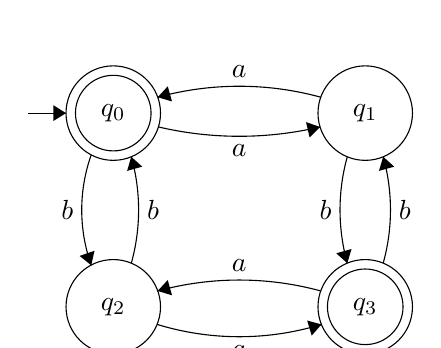
\begin{tikzpicture}[scale=0.2]
\tikzstyle{every node}+=[inner sep=0pt]
\draw [black] (10.5,-13.6) circle (3);
\draw (10.5,-13.6) node {$q_0$};
\draw [black] (10.5,-13.6) circle (2.4);
\draw [black] (26.5,-13.6) circle (3);
\draw (26.5,-13.6) node {$q_1$};
\draw [black] (10.5,-25.9) circle (3);
\draw (10.5,-25.9) node {$q_2$};
\draw [black] (26.5,-25.9) circle (3);
\draw (26.5,-25.9) node {$q_3$};
\draw [black] (26.5,-25.9) circle (2.4);
\draw [black] (5.1,-13.6) -- (7.5,-13.6);
\fill [black] (7.5,-13.6) -- (6.7,-13.1) -- (6.7,-14.1);
\draw [black] (9.103,-23.257) arc (-160.37977:-199.62023:10.443);
\fill [black] (9.1,-23.26) -- (9.31,-22.34) -- (8.36,-22.67);
\draw (8,-19.75) node [left] {$b$};
\draw [black] (11.644,-16.366) arc (15.62592:-15.62592:12.564);
\fill [black] (11.64,-16.37) -- (11.38,-17.27) -- (12.34,-17);
\draw (12.61,-19.75) node [right] {$b$};
\draw [black] (23.72,-27.017) arc (-72.94044:-107.05956:17.792);
\fill [black] (23.72,-27.02) -- (22.81,-26.77) -- (23.1,-27.73);
\draw (18.5,-28.3) node [below] {$a$};
\draw [black] (13.323,-24.893) arc (105.25681:74.74319:19.674);
\fill [black] (13.32,-24.89) -- (14.23,-25.17) -- (13.96,-24.2);
\draw (18.5,-23.7) node [above] {$a$};
\draw [black] (27.64,-16.367) arc (15.56999:-15.56999:12.602);
\fill [black] (27.64,-16.37) -- (27.37,-17.27) -- (28.34,-17);
\draw (28.6,-19.75) node [right] {$b$};
\draw [black] (25.361,-23.132) arc (-164.44592:-195.55408:12.613);
\fill [black] (25.36,-23.13) -- (25.63,-22.23) -- (24.66,-22.5);
\draw (24.4,-19.75) node [left] {$b$};
\draw [black] (23.634,-14.478) arc (-76.79443:-103.20557:22.472);
\fill [black] (23.63,-14.48) -- (22.74,-14.17) -- (22.97,-15.15);
\draw (18.5,-15.57) node [below] {$a$};
\draw [black] (13.322,-12.59) arc (105.31427:74.68573:19.606);
\fill [black] (13.32,-12.59) -- (14.23,-12.86) -- (13.96,-11.9);
\draw (18.5,-11.39) node [above] {$a$};
\end{tikzpicture}
\end{center}
Außerdem sei die folgende Grammatik gegeben: 
\begin{align*}
G = (\{V_0, V_1, V_2, V_3\}, \{a, b\}, P, V_0)
\end{align*}
wobei $P$ auch hier visuell dargestellt wird durch:
\begin{align*}
& V_0 \longrightarrow aV_1~|~bV_2~|~\varepsilon \\
& V_1 \longrightarrow aV_0~|~bV_3 \\
& V_2 \longrightarrow aV_3~|~bV_0 \\
& V_3 \longrightarrow aV_2~|~bV_1~|~\varepsilon 
\end{align*}
\\

a) Zeigen Sie per Induktion über die Länge von Worten, dass $M$ genau die Worte $w \in \{a, b\}^*$ akzeptiert, für die $\#_a(w) \equiv \#_b(w) \pmod 2$ gilt. \\\\
\textit{{\bf Hinweis:} Starten Sie die Induktion bei der Wortlänge 0 und wählen Sie eine sinnvolle Induktionsvoraussetzung! Testen Sie dazu ein paar Beispielworte gerader und ungerader Länge darauf, in welchem Zustand der Lauf des Automaten endet.} \\

b) Zeigen Sie per Induktion über die Länge von Ableitungen, dass $G$ genau die Worte $w \in \{a, b\}^*$ ableiten kann, für die $\#_a(w) \equiv \#_b(w) \pmod 2$ gilt. \\\\
\textit{{\bf Hinweis:} Starten Sie die Induktion bei Ableitungen mit einem Ableitungsschritt und wählen sie eine sinnvolle Induktionsvoraussetzung! Stellen Sie dazu ein paar Ableitungen auf und überlegen Sie sich eine Vermutung, was nach einer gerade bzw. ungeraden Anzahl an Ableitungsschritten gilt. Es gibt eine Analogie zu der Induktionsvoraussetzung in a).} \\

c) Erklären Sie kurz in Worten, inwiefern die Zustände bzw. Transitionen von $M$ den Nichtterminalen bzw. Produktionen in $G$ entsprechen. Unterscheiden Sie bei den Zuständen zwischen Startzuständen, Endzuständen und den restlichen Zuständen. \\

%----------------------------------------------------------------------------------------

\newpage

\section{PÜ 02}

%---------------------------------------------------

\subsection{Reguläre Sprachen}

Geben Sie für folgende Sprachen einen endlichen Automaten an. Sei $\sum = \{ a,b \}$. \\

1.) Alle Wörter, die mindestens 3 a's enthalten. \\

2.) Alle Wörter mit Länge $\leq 5$ \\

3.) Alle Wörter mit Wortlänge kongruent modulo 5. \\

4.) Alle Wörter mit einer geraden Anzahl an a's. \\

5.) Alle Wörter die mit \emph{abaa} beginnen. \\

%---------------------------------------------------

\subsection{Determinisierung}

Lasst die Leute folgende Automaten determinisieren. Achtet darauf, dass die Tupel angegeben werden. Erklärt vorher auch ruhig die Idee, dass die Zustände Mengen von Zuständen des nicht-deterministischen Automaten sind. Erklär auch unbedingt das saubere aufschreiben mit Tabelle wie auf dem Blatt verlangt.

%----------------------------------------------------------------------------------------

\newpage

\section{Übung 03}

%---------------------------------------------------

\subsection{DEA}

Betrachten SIe den folgenden DEA: \\

$A= ( \{ q_{0}, q_{1}, q_{2}, q_{3} \} , \{ a,b \} , \delta , q_{0}, \{ q_{0} , q_{2} \})$ \\

wobei $\delta$ durch folgende Schaubild graphisch dargestellt sei: \\

a) Konstruieren Sie ein Typ-3-Grammatik G, so dass $L(A) = L(G)$ gilt. Verwenden Sie dazu das Verfahren aus der Vorlesung (aus dem Beweis für den Satz aus Folie 47). Denken Sie daran den Automaten zuerst entsprechen zu modifizieren und geben Sie auch das Tupel von G an! \\

b) Beschreiben Sie die Sprache $L(A)$ in einem Satz. \\

%---------------------------------------------------

\subsection{NEA}

Sei $A = (Q, \{ a,b \}, \delta , Q_{0} , F)$ ein NEA (nicht-deterministischer endlicher Automat). Formel akzeptiert ein NEA ein Wort $w=a_{1}a_{2}...a_{n}$ genau dann, wenn eine Folge von Zuständen $q_{0}q_{1}...q_{n}$ existiert mit \\

\begin{itemize}
\item $q_{0} \epsilon Q_{0}$
\item $q_{n} \epsilon F$
\item $(q_{i}, a_{i+1}, q_{i+1}) \epsilon \delta$ für alle $0 \leq i < n$
\end{itemize}  

EIne solche Folge heißt akzeptierender Lauf von A auf w. \\

a)Zeigen Sie: Wenn $Q_{0} = Q$, also alle Zustände auch Startzustände sind, und wenn $w \epsilon L(A)$, dann akzeptiert A auch jedes Suffix von w. \\

b) Zeigen Sie: Es existiert ein NEA A' mit $L(A') = \{ w^{R} | w \epsilon L(A) \}$, wobei $w^{R}$ das Wort w rückwärts gelesen ist. Geben Sie ihre Konstruktion an und beweisen Sie die Korrektheit mit obiger Definition von Akzeptanz. \\

%---------------------------------------------------

\subsection{Automaten}

1.) Sei $\sum = \{ a,b \}$. Geben Sie für $L = \{ w \epsilon \{ a,b \} * $ | das zweitletzte Zeichen von w ist a \} einen DEA (deterministischer endlicher Automat) und einen NEA, der kein DEA ist, an. \\

2.) Die Definition, wann eine DEA ein Wort akzeptiert, ist analog zu der Definition aus Aufgabe 2. Erklären Sie in eigenen Worten wo dennoch Unterschiede liegen. Wie viele akzeptierende Läufe besitzt ein DEA für ein gegebenes Wort höchstens? Wie viele akzeptierende Läufe muss ein NEA für ein Wort besitzen, damit er es akzeptiert? \\

3.) Betrachten Sie die endlichen Automaten, deren Übergangsrelationen in den Abbildungen graphisch dargestellt sind. Geben Sie für jeden Automaten an, ob es sich um einen DEA und/oder einen NEA handelt. Begründen Sie jeweils ihre Entscheidung. \\

%---------------------------------------------------

\subsection{nichtdeterministische Automaten}

a) Im folgenden seien vier nichtdeterministische  Automaten graphisch dargestellt: \\

Konstruieren Sie, mit dem Verfahren aus der Vorlesung jeweils einen deterministischen Automaten, der die selbe Sprache akzeptiert. Verwenden Sie dazu jeweils eine Tabelle. \\

Die Tabelle beschreibt am Ende des Verfahrens die Übergangsfunktion des deterministischen Automaten. Unterstreichen Sie die Endzustände in der Tabelle. Zeichnen Sie außerdem jeweils die Übergangsrelation des entstehenden Automaten und geben Sie das Tupel an. \\

b) Es kann vorkommen, dass eine Zelle in der Tabelle leer bleibt, weil kein Zustand erreichbar ist für eine Kombination aus einer Menge von Zuständen des ursprünglichen Automaten und eines Eingabezeichens. Welchem Zustand der Potenzmengenkonstruktion entsprechen diese Zellen? \\

c) Wie viele Zustände hat ein so konstruierter Automat höchstens, wenn der ursprüngliche Automat n Zustände hatte? Begründen Sie mit höchstens zwei Sätzen! \\

%----------------------------------------------------------------------------------------

\newpage

\section{PÜ 03}

%----------------------------------------------------------------------------------------

\newpage

\section{Übung 04}

%----------------------------------------------------------------------------------------

\newpage

\section{PÜ 04}

%---------------------------------------------------------------------------------------
\end{document}